\documentclass[12pt]{article}
\usepackage[a4paper,top=2cm,bottom=2cm,left=2cm,right=2cm]{geometry}
\usepackage{tocloft}
\usepackage{listings}
\usepackage{graphicx}
\usepackage{wrapfig}
\usepackage{amsmath}
\usepackage{xcolor}
\usepackage{scrextend}
\usepackage{float}
\usepackage{hyperref}
\usepackage{biblatex}
\addbibresource{biblography.bib}

\definecolor{codegreen}{rgb}{0,0.6,0}
\definecolor{codegray}{rgb}{0.5,0.5,0.5}
\definecolor{codepurple}{rgb}{0.58,0,0.82}
\definecolor{codepurpler}{rgb}{0.5 0.0 0.2}
\definecolor{backcolour}{rgb}{0.95,0.95,0.92}
\lstdefinestyle{mystyle}{
    backgroundcolor=\color{backcolour},   
    commentstyle=\color{codegreen},
    keywordstyle=\color{magenta},
    numberstyle=\tiny\color{codegray},
    stringstyle=\color{codepurple},
    basicstyle=\ttfamily\footnotesize,
    breakatwhitespace=false,         
    breaklines=true,                 
    captionpos=b,                    
    keepspaces=true,                 
    numbers=left,                    
    numbersep=5pt,                  
    showspaces=false,                
    showstringspaces=false,
    showtabs=false,                  
    tabsize=2,
    gobble=2
}

\lstdefinelanguage{JavaScript}{
  keywords={break, case, catch, continue, debugger, default, delete, do, else, false, finally, for, function, if, in, instanceof, new, null, return, switch, this, throw, true, try, typeof, var, void, while, with},
  morecomment=[l]{//},
  morecomment=[s]{/*}{*/},
  morestring=[b]',
  morestring=[b]",
  ndkeywords={class, export, boolean, await, throw, implements, import, this, async},
  keywordstyle=\color{magenta}\bfseries,
  ndkeywordstyle=\color{codepurpler}\bfseries,
  identifierstyle=\color{black},
  commentstyle=\color{codegreen}\ttfamily,
  stringstyle=\color{codepurple}\ttfamily,
  sensitive=true
}
\lstset{style=mystyle}
 
\renewcommand{\cftsecleader}{\cftdotfill{\cftdotsep}} % for dots in table of contents for sections

\newcommand{\code}{\texttt} 

\begin{document}
\setlength{\baselineskip}{1.5\baselineskip} % This sets the line spacing to something that looks like 1.5 in Word

\begin{titlepage} % Suppresses displaying the page number on the title page and the subsequent page counts as page 1
	\newcommand{\HRule}{\rule{\linewidth}{0.5mm}} % Defines a new command for horizontal lines, change thickness here
	
	\center % Centre everything on the page
	
	%------------------------------------------------
	%	Headings
	%------------------------------------------------
	
	\textsc{\LARGE University of Southern Denmark}\\[1.5cm] % Main heading such as the name of your university/college
	
	\textsc{\Large Computer Science}\\[0.5cm] % Major heading such as course name
	
	\textsc{\large BADM500 - Bachelorprojekt i datalogi}\\[0.5cm] % Minor heading such as course title
	
	%------------------------------------------------
	%	Title
	%------------------------------------------------
	
	\HRule\\[0.7cm]
	
	{\huge\bfseries Karatsuba and Curve22519 on RISV-V }\\[0.3cm] % Title of your document
	
	\HRule\\[1.5cm]
	
	%------------------------------------------------
	%	Author(s)
	%------------------------------------------------
	\begin{minipage}[c]{0.5\textwidth}
		\begin{flushleft}
			\large
			\textit{Author}\\
			[5mm]
			{Michael Saabye Salling \\}
			{misal18}\\
			{29-01-1994}\\
			\textsc{\Large }\\
			\end{flushleft}
	\end{minipage}
	~
    \begin{minipage}{0.4\textwidth}
		\begin{flushright}
		\large
  		\kern1.0cm
  		 \raggedleft
  		\textit{Supervisor}\\
  		\kern+0.5cm
		Ruben Niederhagen\\
		\large
  		\kern-4.5cm
  		 \raggedleft
  		\textit{External censor}\\
  		\kern+0.5cm
		Claudio Orlandi\\
		\end{flushright}
	\end{minipage}\\
	[6cm]
	
	% If you don't want a supervisor, uncomment the two lines below and comment the code above
	%{\large\textit{Author}}\\
	%John \textsc{Smith} % Your name
	
	%------------------------------------------------
	%	Date
	%------------------------------------------------
	
	\vfill\vfill\vfill % Position the date 3/4 down the remaining page
	
	{\large{\today}} % Date, change the \today to a set date if you want to be precise

	
	\end{titlepage}
	\clearpage

    \pagenumbering{gobble} %disable page numbering
    \tableofcontents
    \clearpage
    \pagenumbering{arabic} %enable page numbering
    
    \section{Abstract}
I denne rapport vil jeg gennemgå hvordan Karatsuba er blevet brugt til at optimere udregningerne brugt i curve 22519. Karatsuba er en hurtig multiplikations algoritme som kan bruges til store integer værdier.\\En reference implementation af curve 22519 er blevet ported til RISC-V og bliver simuleret på PQVexRiscV CPU'en. En evaluering af optimeringe er gjort udfra test resultaterner som kommer fra programmer der kører på en simuleret CPU.
	\section{Introduction}
 2 pages
Introduce platform, curve / scheme (1 page), background about riscv (2-3 page)\\
\\
A essential part of computing is having a secure cryptographic algoritm. Theese algoritms has become a crucial part of messaging, and network systems.
The goal of this project is to port Curve25519 to RISC-V, and optimize it for the VexRiscv platform.
\\
Curve25519 is a elliptic cure algoritm released by Daniel J. Bernstein in 2005. The algorithm was originally defined as a Diffie-Hellman function.
ECC uses smaller keys than RSA while providing the same level of security, with faster key generation.
A ECC public key contains a pair of integer coordinates \textit{(x, y)} on the curve. A elliptic point can be compressed to a single X coordinate, which is used by curve 25519.
\\
The Elliptic-curve Diffie-Hellman is a key agreement scheme, which allows two parties to establish a shared secret with 2 different public/private key sets. 
Eliptic-curve Diffie-Hellman (ECDH) is very similar to a classical Diffie Hellman, the difference is that ECDH uses \textit{ECC point multiplication} where the classical approach uses \textit{modular exponentations}.
\pagebreak
	\section{Background}


\subsection{Scheme}
(~ 1 page)


\subsection{RISC-V}
(~ 1 page)
The RISC-V ISA is a open standard instruction set which is free and uses a open license. The license allows for development of closed and opensource implemenations for commercial and non-commercial use.

A reduced instruction set computer (RISC) `?????????'


Instruction set architecture (ISA) defines the the instructions which the architecture must support. A ISA also specifies instructions for handling data and memory operations, and how data id encoded in the registers.

The RISC-V ISA has modular design with different ISA bases which defines instructions for integers and weak memory ordering, and a number of extensions developed in a collective efforts with researchers and companies.
A modular approach allows the implementors to disable extension which is not needed, and save money on space and power used. 
Extensions are activeley being developed, with some being in a "frozen" state. Which is defined as not expected to change during the ratification proccess.

A company might not find the extensions they need for their product. In that situation a custom ISA extension can be used, to add their special instructions. 
This dosent break the compliance with the main specification, which means that software made for the main specification will still work on the extended ISA.

https://riscv.org/wp-content/uploads/2017/05/riscv-spec-v2.2.pdf
https://riscv.org/about/faq/
https://www.design-reuse.com/articles/46237/extending-risc-v-isa-with-a-custom-instruction-set-extension.html
	\section{Optimization}
~10 pages


-- Skriv om hvor der ELLERS kunne optimeres??


\subsection{Karatsuba}
The Karatsuba algorithm is used to perform multiplication of large numbers with fewer operations, than the school-book multiplication approach.
$n^{\log_{2}3} \approx n^{1.58}$
As multiplication is a 

Multiplication is used intensly during the encryption[] steps, this was a focus of optimization. The reference implementation of the curve uses simple schoolbook multiplication.
Where every single digit is multiplied with the corresponding digit in the other number, and a carry is carried on to the next iteration when the result is bigger than the base. This carry will then be multiplied with the next set of digits.\\
EXAMPLE IMAGE\\
The schoolbook approach requires $n^{2}$ single-digit products. 
This approach is the approach used in the reference implemention, which can be replaced with a more optimal algorithm.
\\

The Karatsuba algorithm 
\label{karat-opti}
\[A_0 \times B_0 + 2^{m}((A_0 + A_1) \times (B_0 + B_1) - A_0 \times B_0 - A_1 \times B_1) + 2^{2m} A_1 \times B_1\]
This approach requires 5 products, with 2 of them being the same multiplications. For this reason 2 of them can be stored and them re-used without any calculations.
\\EXAMPLE IMAGE\\
The Karatsuba algorithm uses more additions compared to the schoolbook approach which uses 4 multiplications and 3 additions, this uses 3 multiplications, 4 additions and 2 subtractions. So the algorithm saves multiplications at the cost of additions and subtractions. Thus is Karatsuba faster if multiplication is more expensive than additions and subtractions. 


	
	\section{Implementation}
    crucial arithmetic
    How it works together
    Reference ideas (Maybe from litterature)
    - Explain how you got th idea
    - Did you get the idea from somewhere else, explain it from where
	
	\section{Evaluation}
	Around 2 - 3 pages
    - Reference implementation
     * Base reference
    - Testing, and how it was done
    - Different stages of implementations
    - Compare
-----



An evaluation can me made using the data gotten using the test scripts described in the implementation section. All measurements is measured by counting the cycles it takes to run the code.

\subsection{Testing}



\subsection{Reference implementation}
The reference implementation uses Montgomery ladder approach for point multiplication, schoolbook multiplication, and branch less fixed time approaches to the arithmetic in general. This makes it easier to measure the cycles as it they wont change depending on its input. The reference implementation takes $79.898$ megacycles to run.

\subsection{Karatsuba}
The testing method described in \ref{karatTesting} has been used to find the best operand length for the Karatsuba algorithm. The results of the test scripts has been plotted into a chart, and can be seen in figure \ref{karatsubafigure}. Based on those results the best operand length must be $32$, as this results in the least cycles. \\ 
\begin{figure}[H]
\begin{subfigure}{\textwidth}
    \centering
    \fbox{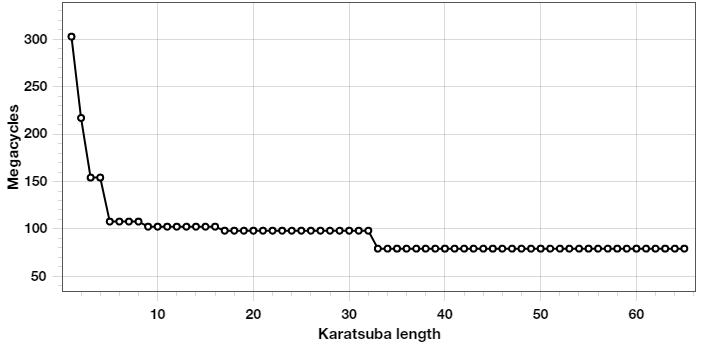
\includegraphics[width=0.8\textwidth]{report/images/karatsuba.png}}
    \caption{Karatsuba operand length - cycles}
\label{karatsubafigure}
\end{subfigure}
\end{figure}
Using this operand length results in $79.222$ megacycles. To compare the Karatsuba cycles with the reference implementation both have been plotted into a chart in figure \ref{karatsubacomparison}. This chart shows the difference between the two implementation is not magnificent, as the difference is $0.676$ megacycles.\\

\begin{figure}[H]
\begin{subfigure}{\textwidth}
    \centering
    \fbox{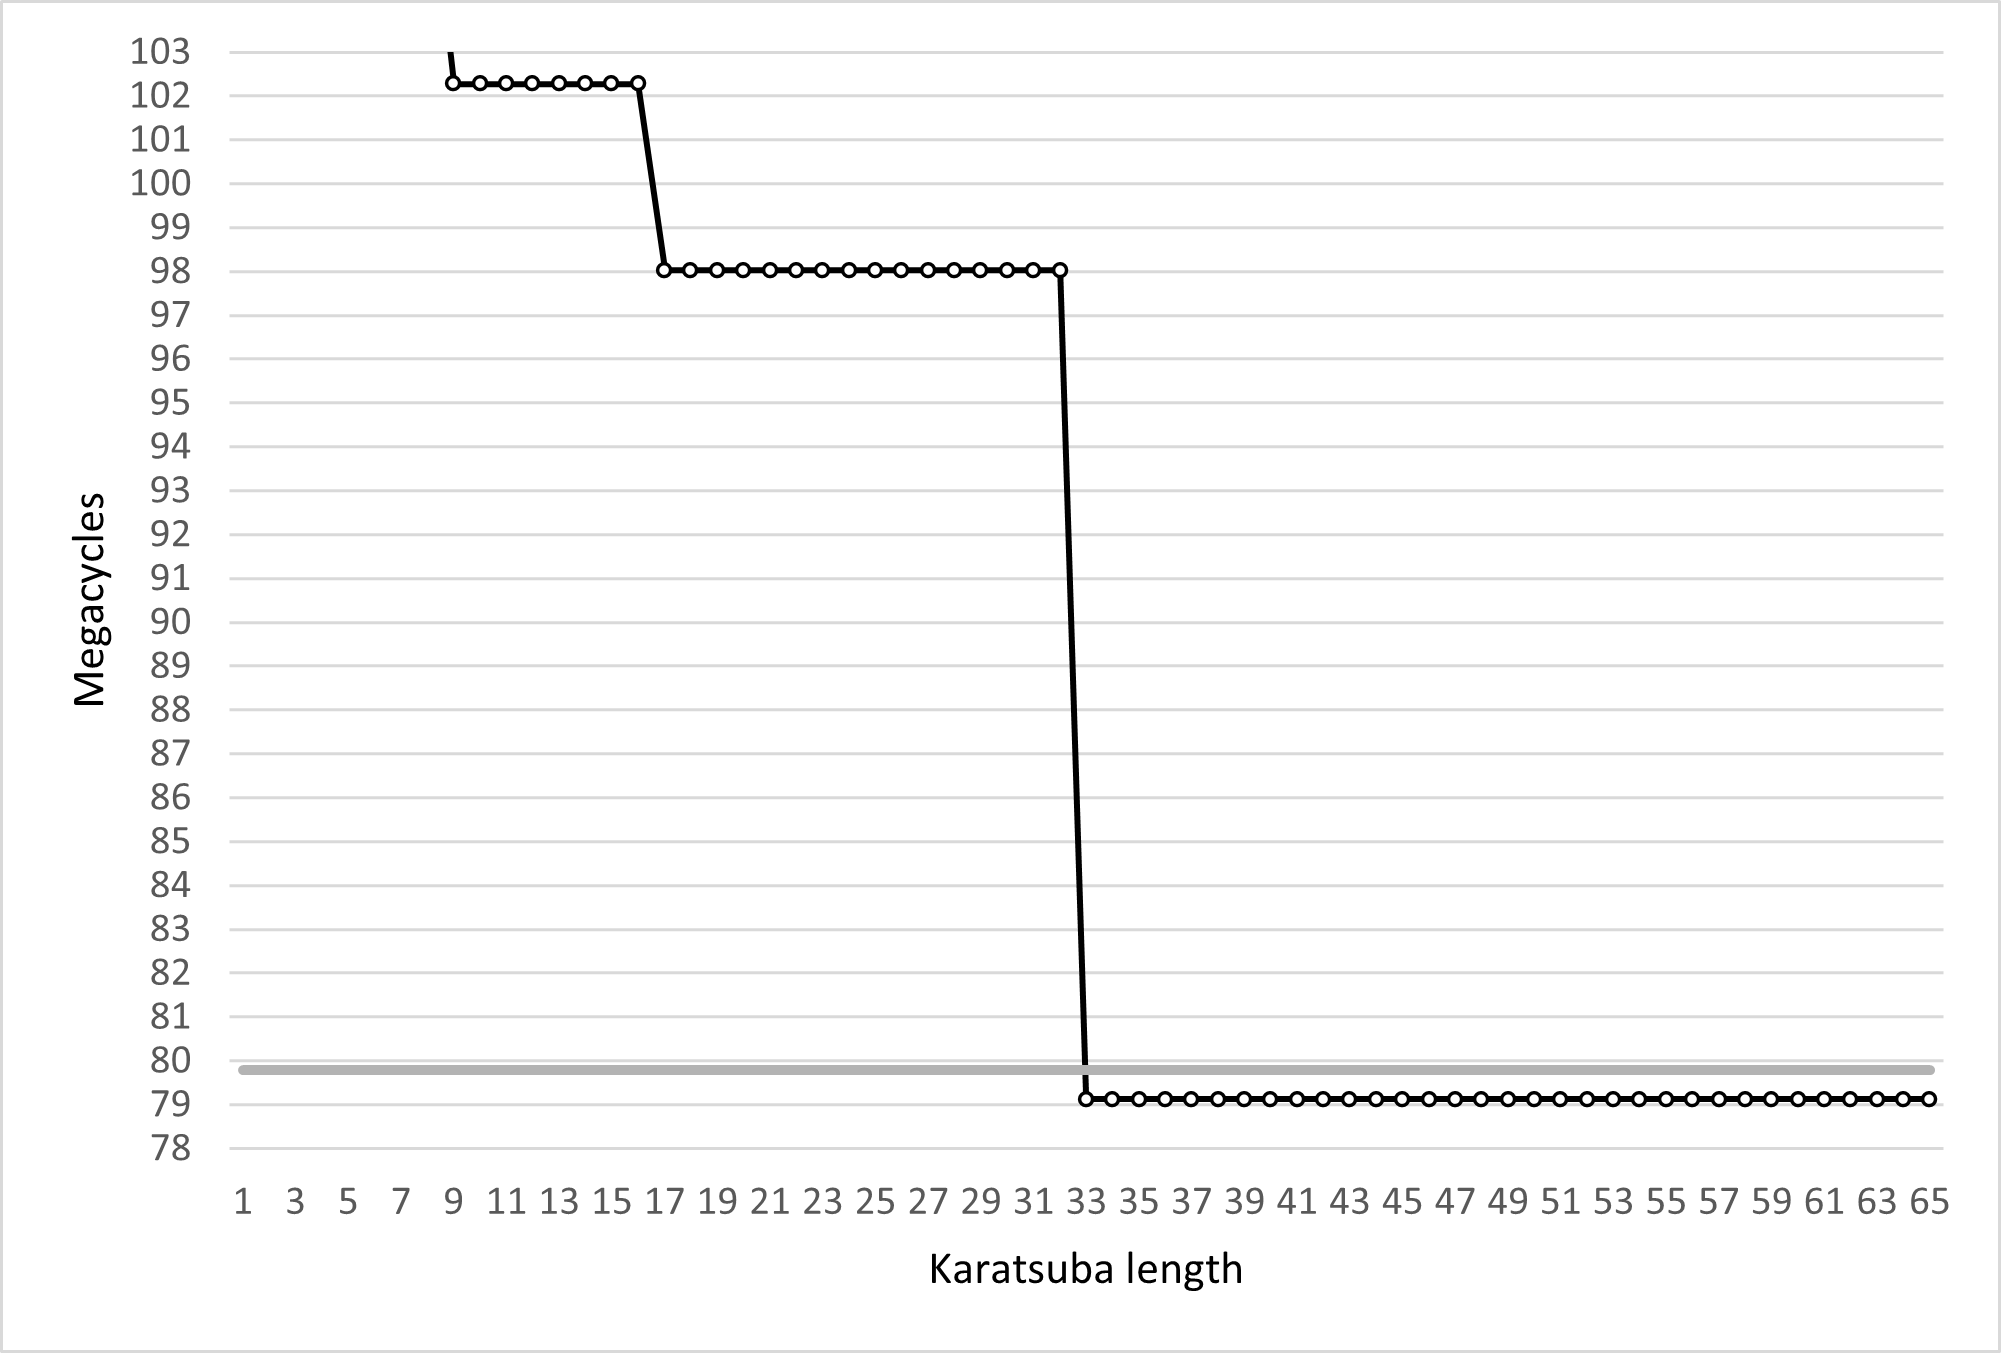
\includegraphics[width=0.8\textwidth]{report/images/karatsuba-compared.png}}
    \caption{Karatsuba operand lengths compared to reference implementation}
\end{subfigure}
\label{karatsubacomparison}
\end{figure}
    
	\section{Conlusion}
% 1 page
The goal of this project was to port was to setup a simulation of the RISC-V ISA using the platform
VexRiscv. Then port a reference implementation of Curve22519 to this platform, and optimize and evaluate the optimizations. \\
A small optimization to the multiplication arithmetic was the only thing implemented due to time constraints. The Karatsuba algorithm implemented is only a nominally amount faster compared to the reference implementation. This could however be a good foundation for further optimizations, or other kinds of multiplication algorithms. A lot of time was used to understand what exactly was going on, and how everything works together in the reference implementation.\\
It is difficult to determine the correctness of the changes due to the scope of the project, but does seem like it works as intended from the testing and comparisons that has been done with the reference implementation.\\
The overall project was successful, even though it wasn't significant improvements in cycles.

    \printbibliography

    \clearpage     
\end{document}